% !TEX root = ../../thesis.tex

% \cleardoublepage
% \newpage
% \thispagestyle{plain}
% \mbox{}

% \includepdf{/Users/matthieulapeyre/Documents/phd_thesis/media/poppy.pdf}
% \includepdf{/Users/matthieulapeyre/Documents/phd_thesis/media/blueprint}

\chapter{The Poppy development} % (fold)

\section{Motivations} % (fold)

\begin{figure}[!b]
\centering
    \subfloat[][Nao]{\label{fig:knee_wout_spring}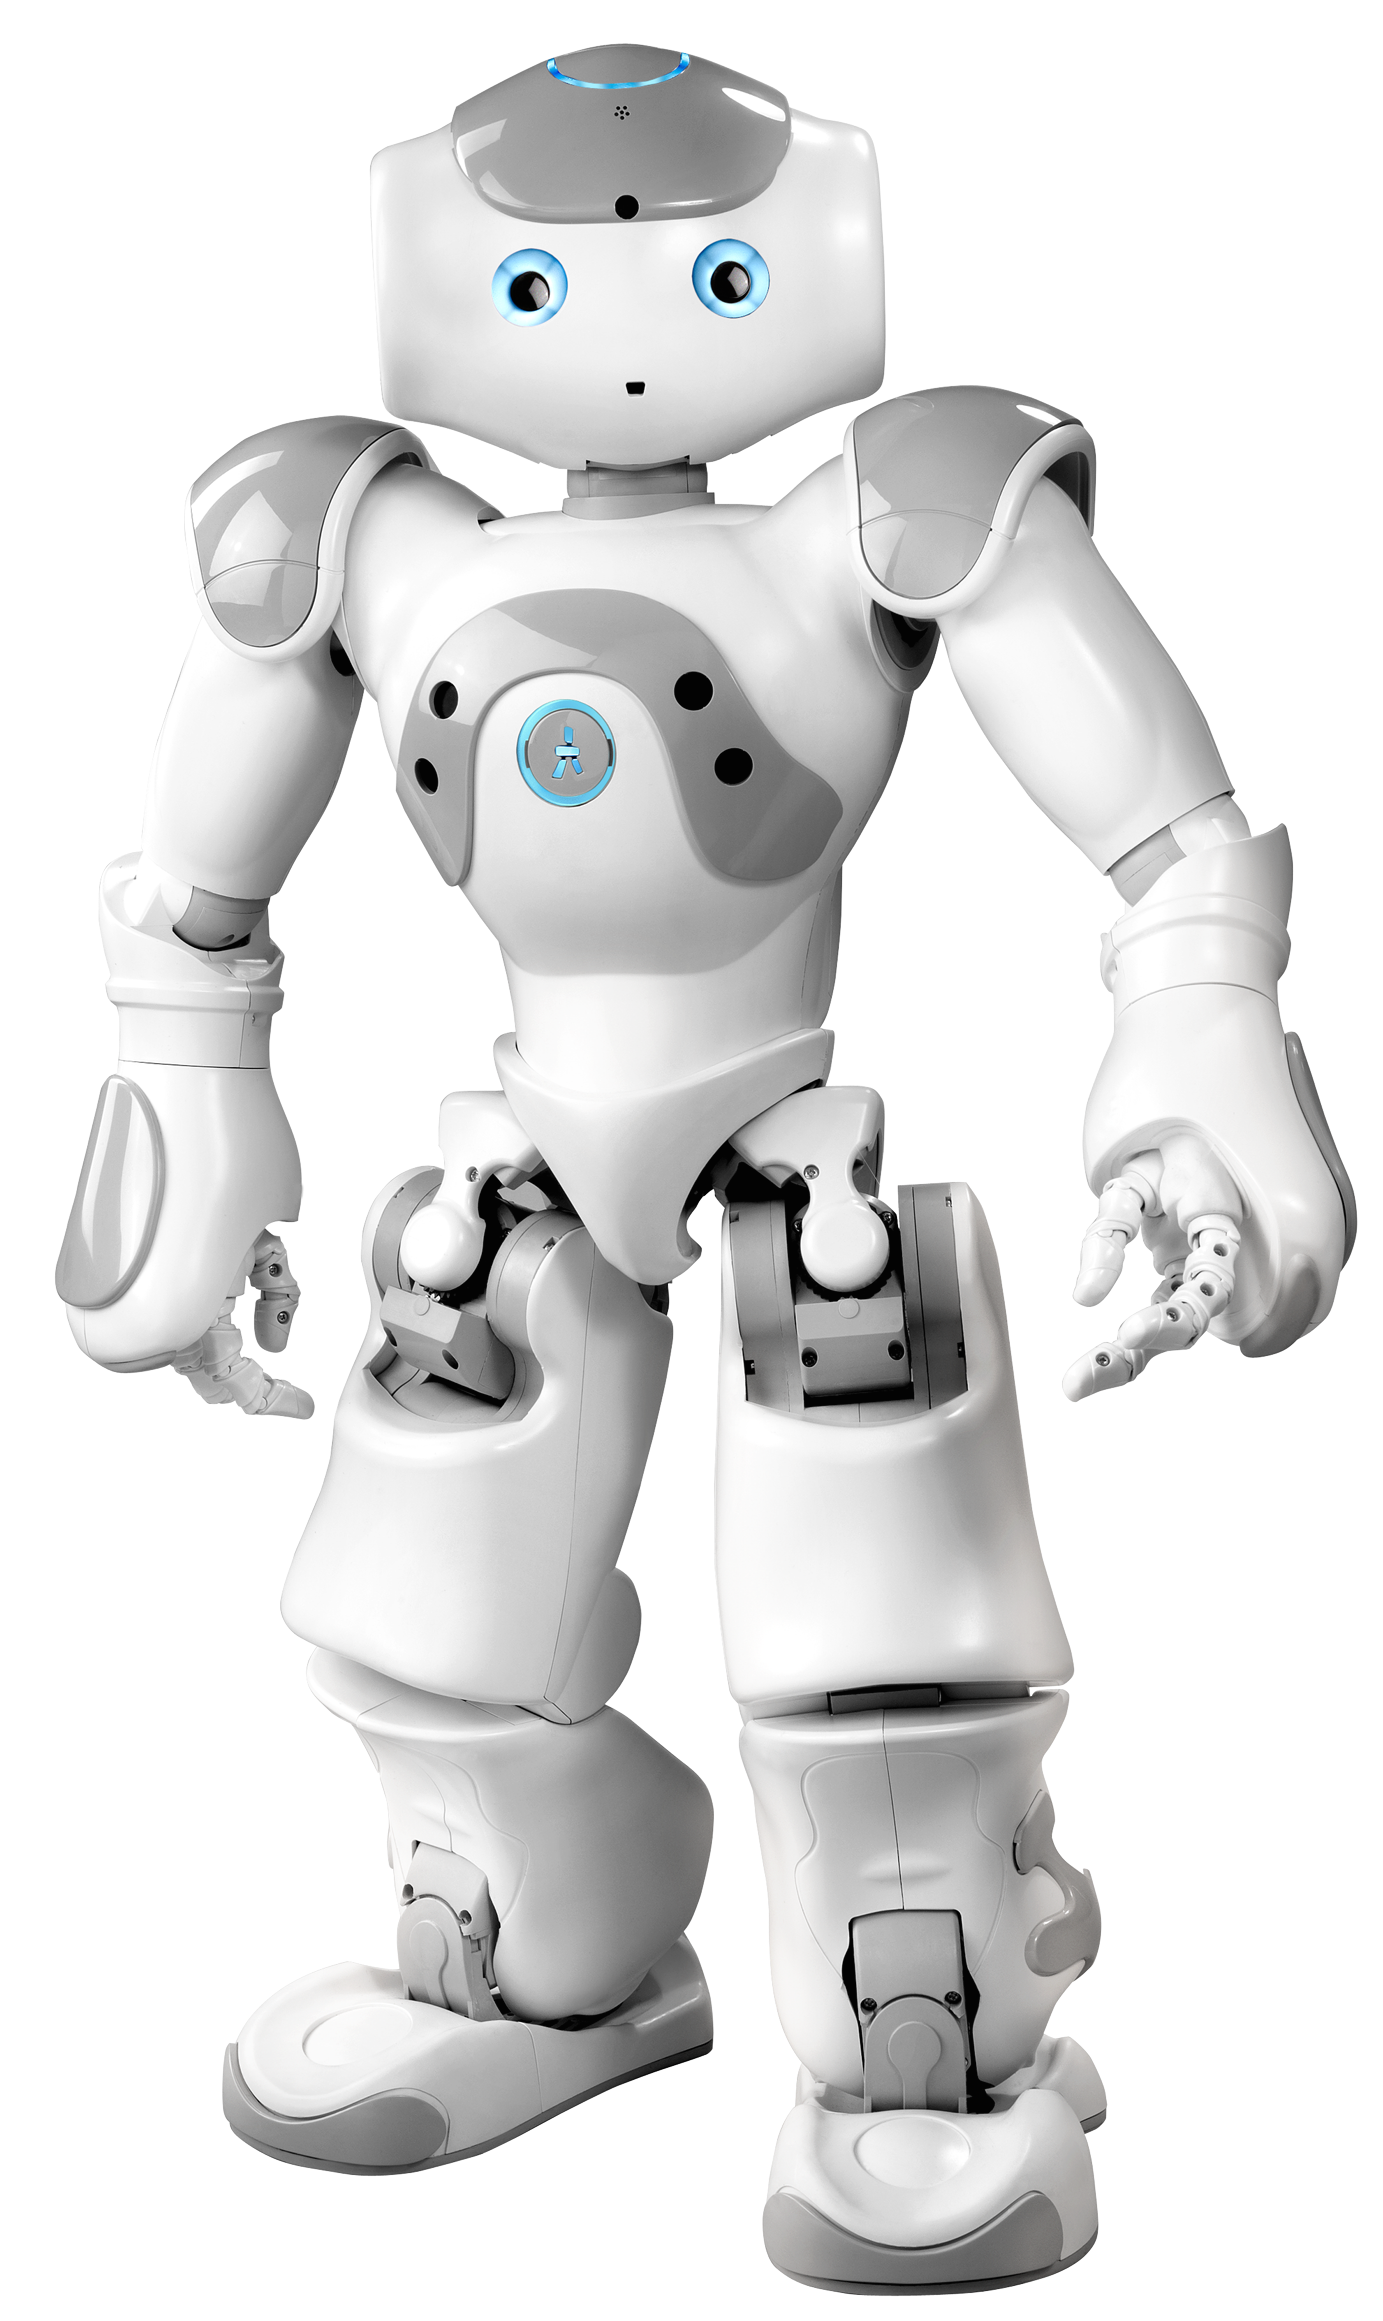
\includegraphics[height=5cm]{nao_face.png}}
    \hfil
    \subfloat[][Darwin-Op]{\label{fig:knee_w_spring}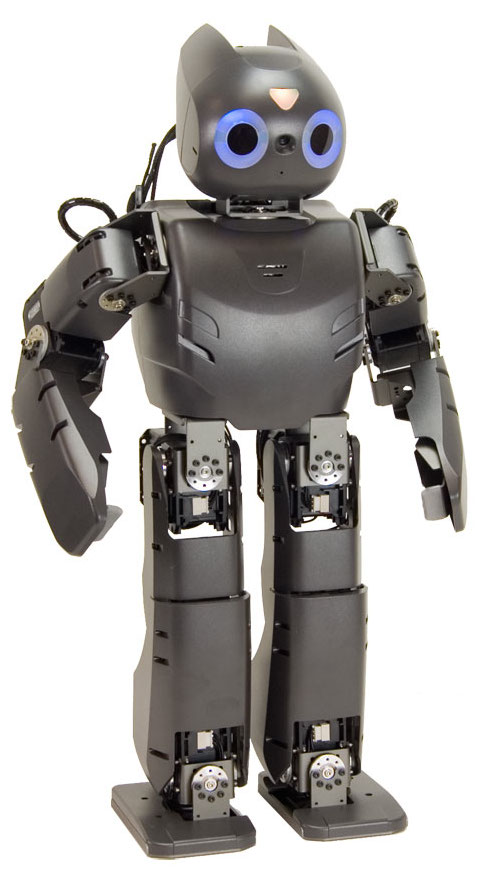
\includegraphics[height=5cm]{darwin_op_face.jpg}}
    \hfil
    \subfloat[][Acroban]{\label{fig:acroban}\includegraphics[height=5cm]{acroban_wout_background.jpg}}
    \caption{None of the existing platform in 2012 was suitable to explore the role of morphology. Nao was impossible to modify. Darwin Op and Acroban used aluminium part really difficult and expensive to produce.}
    \label{fig:2012_Humanoids}
\end{figure}

In this thesis we are interested in the role of morphology, especially concerning the biped locomotion. Indeed, as we discussed in the chapter REF, the robot morphology can be a way to make robot easier to control and more adapted to their environmental niche. For this purpose, exploring principles such as morphological computation, soft robotics or passive dynamics seems to be an fantastic and promising open field of research for both designing more efficient and intelligent humanoid robot, and better understanding animal's behavior, Human being in particular.

However exploring these concepts require embodiment. Experimentations have to be in the real world because we need to provoke emergence. In addition, exploring the morphology means we should consider morphology as an experimental variable, i.e we should design, build and experiment morphological variation of the actual robot body.

When we began this work (mid-2012), no other robotic platform allowed to easily explore morphological variants (sse \figurename~\ref{fig:2012_Humanoids}). Most of them had a classical conception i.e. rigid and high-power actuation and had a structure made of either plastic or aluminum parts.  , the ones interesting were lab prototype and were not reproducible.

Following the work introduced with Acroban, we decided to develop a whole new humanoid platform using the methodology we discussed in the previous chapter. Poppy\texttrademark has been the first 3D printed and open source (software \& hardware) complete-humanoid robot.


Thus we decided to extend the ability of Poppy to the exploration a wider range of scientific challenge such as Human Robot Interaction (HRI), sensorimotor learning, ...
Allowing the Poppy platform to raise its ambition to become a benchmarking platform.

Thanks to our FabLab-inspired approach, the first functional and diffusible prototype has been achieved in just 4 months.
Then a second version occurred to make the robot more versatile and easy to use for non-expert user such as the education and artistic communities.

In this chapter, we will explain the design of Poppy from both a conceptual and a technical point of view.

With Poppy we decided to build a platform which of course allows to use classic stuff but enable


\section{Poppy overview} % (fold)



gne
Poppy is a robotic platform designed to explore, create,

Poppy allows to explore both morphology and control variants and so how they interact with each other.

Some choice are made to impose a certain way, for example the robot is underactuated then

Poppy c'est une platform de recheche en robotique.

L'impression 3D est un point cles car il permet d'explorer facilement et rapidement differente forme

La platform vise plusieurs domaines:
La recherche en proposant une platform open source permettant un libre echange des resultats entre laboratoire et la comparaison
et pour la première fois la possibilité de partager des resultats hardware.

Pour l'éducation car Poppy


\section{Design guidelines} % (fold)

\subsubsection{Modular morphology} % (fold)
The whole structure must be easy to reconfigure both for repairing or hacking purpose. This mean the process to replace a Poppy's parts must be simple, low-cost and not require time or special tooling.


\subsubsection{Less is more: keep it simple}

The fact we want to design an easily reproducible robot means we are limited in our design choices.
In most case, finding a simple solution avoid the use of an easy solution: we should minimize the number of part and suppliers, be careful of the availability of our parts in each country, take in account the cost and the assembly complexity.
All these constraints make the design of the robot way more complex than a unique prototype robot.
It also raises some limitation to the main Poppy version while some interesting or efficient solution cannot be kept due to their complexity.


\subsubsection{A lightweight structure and under-actuated} % (fold)

Many humanoid robots use powerful motors often associated with highly accurate sensors.
This has a cost, both in terms of weight and computation resources.
Moreover, to ensure the accuracy of the sensory-motor space it is necessary to design very rigid mechanical parts.
The whole structure obtained is powerful but very heavy and due to inertia not very agile.
This kind of robots can intensively repeat precise and complex movements, but are somewhat uncomfortable when it comes to walking on uneven ground.

All mechanical parts were designed to optimize their weight and make the platform Poppy as light as possible.
The obtained mass reduction allows the use of less powerful motors which are therefore lighter.
We can thus have a lightweight robot, strong and powerful enough to perform tasks such as walking and physical interaction.


\subsubsection{Bio-inspired morphology} % (fold)
Human being is a great example of biped locomotion ability.
Strictly mimicking the human morphology is certainly not a good idea as the element composing a robot are not comparable.
However, studying the functional interest of certain human bio-mechanic properties can reveal interesting insight to explore novel humanoid design.

\subsubsection{Ecological balance principle} % (fold)
The ecological balance principle, introduce by Rolf Pfeifer, states that there is a balance or task distribution between morphology, materials, control, and interaction with the environment.
Following this principle, we try to keep a balance between the different part of the robot.

\subsubsection{Whole body compliance} % (fold)
Important aspects of adaptation to physical obstacles or HRI require humanoid robots to be full-body compliant.
This includes both the ability to absorb external shocks due to the passive compliance of the mechanical structure (bendable materials and springs), but also the ability to actively and dynamically control the compliance of motors, which may be either controlled in position with compliance, or directly in torque (thanks to the use of adequate recent servomotor technologies).

\subsubsection{Take care of the aesthetic} % (fold)
In the scientific community, design and aesthetic are often left aside as a superficial feature.
But when an object has to interact with human, the design and aesthetic are the communication channels.
The interaction with our senses change the way we understand the purpose of a object.

As any communication tool, the message we convey can be noised or enforced by the form.
Thus the robot appearance must fit the robot abilities and try to give insights to the user about what it can or cannot do.

Both at a macro or micro scale, the Poppy aesthetic is thought to show some conceptual aspects of its design.
\begin{itemize}
    \item Modular
    \item Smooth and compliant
    \item Lightweight
    \item Under-actuated
\end{itemize}

We do not hide the stuff, user can see motors, wire...



\section{Poppy overview} % (fold)

\begin{figure}[tb]
    \begin{center}
        \includegraphics[width=0.95\linewidth]{poppy-overview.pdf}
    \end{center}
    \caption{Caption here}
    \label{fig:poppyv0.1_overview}
\end{figure}

\begin{figure}[tb]
    \begin{center}
        \includegraphics[width=0.95\linewidth]{poppy-overview-v1.pdf}
    \end{center}
    \caption{Caption here}
    \label{fig:poppyv1_overview}
\end{figure}

Poppy (Fig.~\ref{fig:Poppy_comparaison}) is a 84cm high humanoid robot which weights 3.5kg.
It has a sensorimotor space consisting of 25 motorized joints using Robotis Dynamixel servomotors (MX-28 and AX-12).
These servo-motors give access to a large number of internal sensors and allow tuning dynamically their compliance (see \ref{ssub:robot_actuation}).
The sensors space is extended by the addition of 8 force sensors under each foot, an inertial measurement unit located in the head and two wide-angle HD cameras.
In addition, a 4" LCD screen is located on the face for visual communication (such as emotions, interaction).


In order to develop an adapted mechanical structure, we interested ourselves in how evolution solved sensorimotor task related to locomotion and in particular bipedal locomotion.
As human locomotion represents one of the finest example of mastering bipedal walking, we took functional inspiration of some elements that seem relevant to improve the locomotion of humanoid robots.

\begin{figure}[thpb]
    \centering
    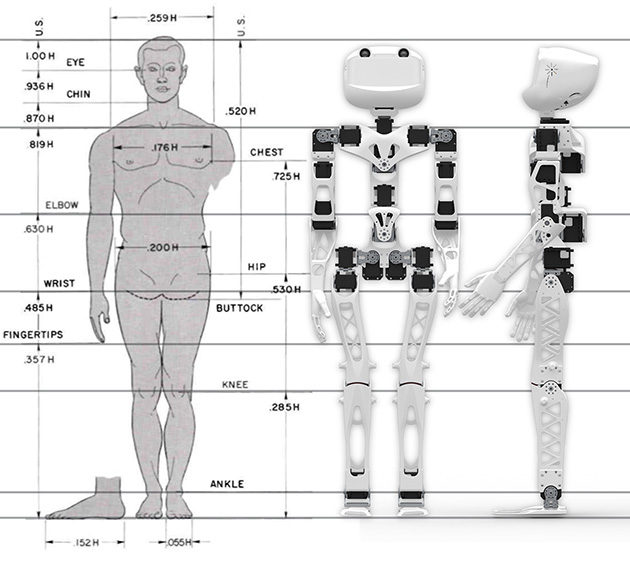
\includegraphics[width=0.9\linewidth]{proportion_poppy.jpg}
    \caption{Human proportion used for the design of Poppy \cite{dufour2005biomecanique}}
    \label{fig:proportion_poppy}
\end{figure}

This bio-inspiration is expressed on the whole structure of Poppy.
On the anatomical point of view, it reproduces the human proportions as described in the literature \cite{dufour2005biomecanique}  (see Fig.~\ref{fig:proportion_poppy}) and their sensorimotor space organization: i.e.
the main degrees of freedom (actuated and passive), an inertial unit in the head and force sensors distributed underfoot.

As explained in \ref{sec:introduction}, biped locomotion is a central design goal of the Poppy platform.
For this purpose, the morphological optimization is mainly expressed on the locomotive system (legs and trunks) in order to increase the robot robustness, agility and stability during the walking.


\subsection{Lightweight and compliant structure} % (fold)
\label{sub:a_ligthweight_and_compliant_structre}
Many humanoid robots use powerful motors often associated with highly accurate sensors.
This has a cost, both in terms of weight and computation resources.
Moreover, to ensure the accuracy of the sensory-motor space it is necessary to design very rigid mechanical parts.
The whole structure obtained is powerful but very heavy and so not very agile.
This kind of robots can intensively repeat precise and complex movements, but are somewhat uncomfortable when it comes to walking on uneven ground.

Following ecological principles \cite{pfeifer2005new} we decided to design a lightweight and compliant robot requiring low actuation power.
All our design choices, such as the materials, the motors or the sensors, have been made in this direction and to try to tackle the challenges presented in the introduction.
In the next sections we will detail each part of the robot and how they fit within these designs principles.

Weight reduction was achieved through the use of trellis structures.
These structures, mainly used in civil engineering, are among the best technical solutions to optimize the weight/resistance ratio.
All the limbs of Poppy are based on this structure and have been optimized using finite element analysis (FEA) to perform structural simulation and validate parts performance and safety factors.


\subsubsection{Actuation} % (fold)
\label{ssub:robot_actuation}
However these motors are quite heavy (72, 126 and 153g respectively for MX-28, MX-64 and MX-106) in comparison of the Futaba servo-motors\footnote{\url{http://www.futaba-rc.com/servos/brushless.html}}, 20-50g for a comparable output torque. Given these constraints, the challenge consists in minimizing the number of motors and the power needed to reduce the global weight of the robot.

% subsubsection robot_actuation (end)

\subsubsection{Material properties} % (fold)
\label{ssub:material_properties}

All mechanicals parts are made using laser sintering technology. This 3D printing process allows the production of almost any shape without constraint. In addition, the price of the part depends on the total size and not on the complexity of the shape. This permits the production of very optimized shapes without increasing the total price of the robot. Also, this technique is compatible with several materials from polyamide to titanium. Parts manufacturing was subcontracted to an external company\footnote{\url{http://i.materialise.com/}}.
For Poppy's structure we decided to use the polyamide material because it is lightweight and very flexible while keeping good strength properties (see the table \ref{tab:materials}).

\begin{table}[h]
    \centering
    \begin{tabularx}{0.8\linewidth }{l X X X}
        Material & Mass Density $\rho$ ($kg/m^3$) &  Yield strength $\sigma$~($MPa$) & Young Modulus $E$($GPa$)\\
        \hline
        Polyamide & $930$ & $49$ & $1.65$\\

        Aluminum & $2700$ & $200$ & $70$\\

        Steel & $7500-8000$ & $350$ & $200$\\

        Titanium & $4500$ & $1200$ & $114$\\

    \end{tabularx}

    \caption{Comparison of material properties.
    The Young modulus represents the stiffness of the material while the yield strength corresponds to the maximal stress tolerable before plastic deformation.}
    \label{tab:materials}
\end{table}


% subsubsection material_properties (end)


\subsubsection{Structure design} % (fold)
\label{ssub:structure_design}


All mechanical parts were designed to optimize their weight and make the platform Poppy as light as possible.
The obtained mass reduction allows the use of less powerful motors which are therefore lighter.
We can thus have a lightweight robot, strong and powerful enough to perform tasks such as walking and physical interaction.

Weight reduction was achieved through the use of trellis structures.
These structures, mainly used in civil engineering, are among the best technical solutions to optimize the weight/resistance ratio.
All the limbs of Poppy are based on this structure and have been optimized using finite element analysis (FEA) to perform structural simulation and validate parts performance and safety factors.


\begin{figure}[!h]
\centering
    \subfloat[][Section of the Poppy's leg]{\label{fig:Poppy_leg_section}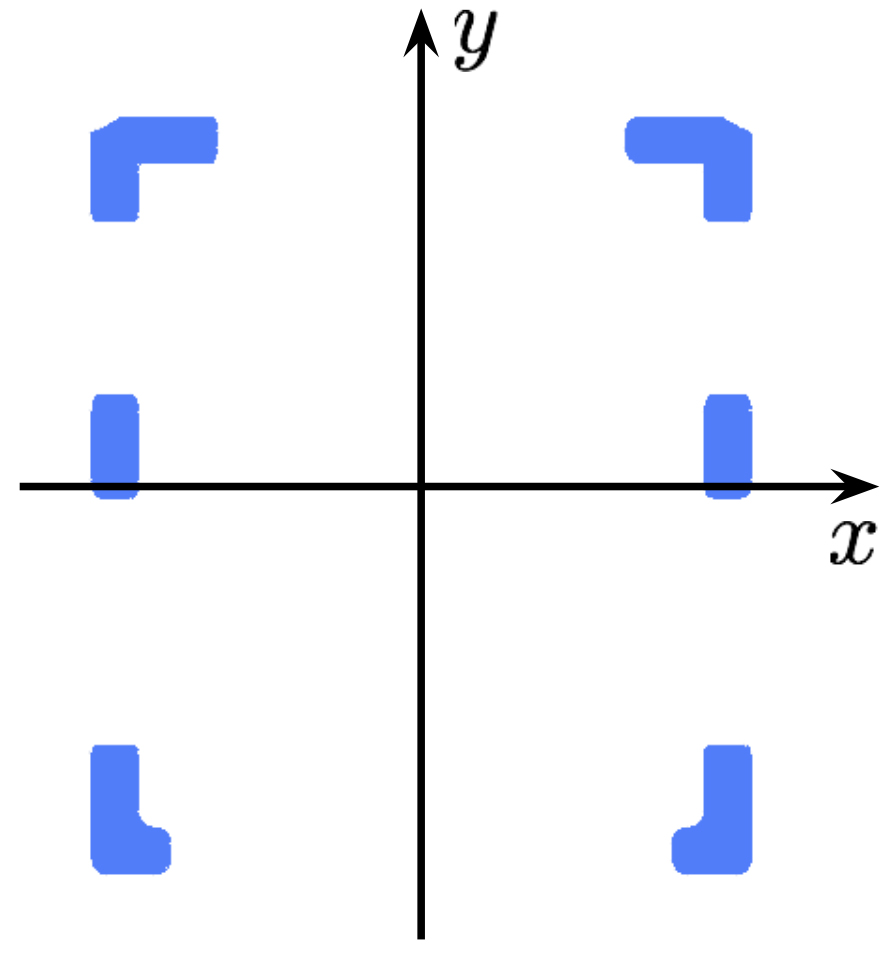
\includegraphics[height=4cm]{Poppy_leg_section.jpg}}
    \hfil
    \subfloat[][Equivalent square section]{\label{fig:basic_leg_section}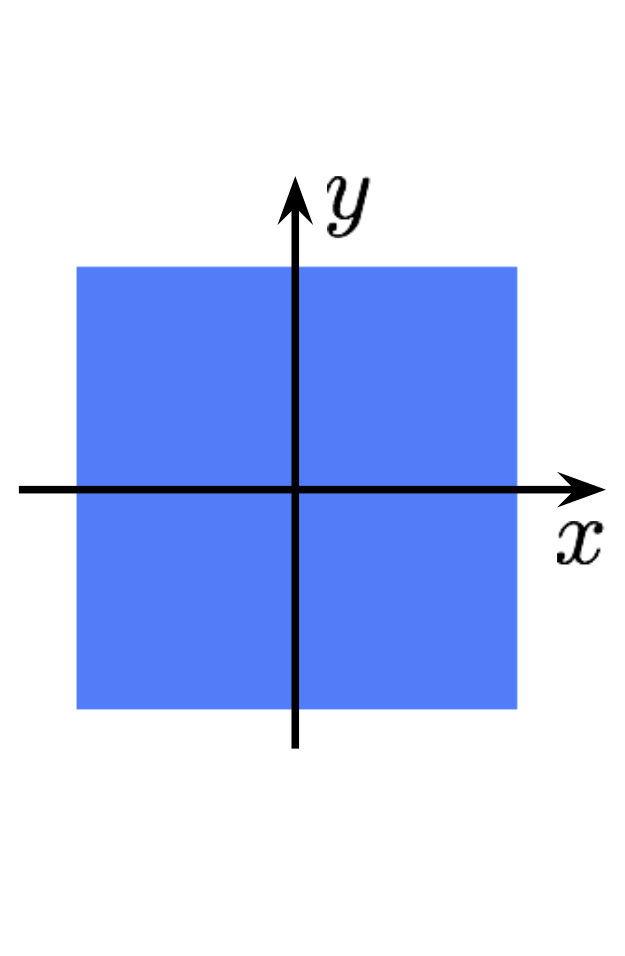
\includegraphics[height=4cm]{basic_leg_section.jpg}}
    \caption{}
    \label{fig:leg_section}
\end{figure}


The main quadratic momentum taken at the middle of the leg given the trellis structure (see Fig.~\ref{fig:leg_section}.a) is:

\begin{center}
    $I_x = \iint_s y^2 dxdy$ and  $I_y = \iint_s x^2 dxdy$

    with $s = dxdy$
\end{center}
\begin{center}
    $I_x = 54.862 mm^4$
    ,
    $I_y = 53.260 mm^4$
\end{center}

For instance, given a solid bar with rectangular profile (Fig.~\ref{fig:leg_section}.b):

{\centering
    $I_x = \frac{b \cdot h^3}{12}$
    ,
    $I_y = \frac{b^3 \cdot h}{12}$
}
It would require a section such as $b=27.72 mm$ and $h=27.59 mm$ to get the same quadratic momentum.
Considering the length of the leg part (i.e.
$190 mm$), the total mass would be equal to $142 g$ instead of $47 g$ for the actual leg.
This corresponds to a reduction of 70\% of the mass.

By using this mesh structure on most of the robot, the total weight of the 3D
printed parts were reduced of about 1.3kg while still being resistant under shocks and falls.


\subsection{The materials} % (fold)
All mechanicals parts are made using laser sintering technology.
This 3D printing process allows the production of almost any shape without constraint.
In addition, the price of the part depends on the total size and not on the complexity of the shape.
This permits the production of very optimized shapes without increasing the total price of the robot.
Also, this technique is compatible with several materials from polyamide to titanium.

For Poppy's structure we decided to use the polyamide material because it is lightweight and very flexible while keeping good strength properties.

\subsection{The actuation} % (fold)

While emerging technologies such as linear motor, artificial muscle or using both motors and cables are promising, they are still not ``plug'n'play'' solutions (e.g.
require air circuit, associating motor and cable is a complex task, pistons are heavy and slow).
It makes their integration in a small platform such as Poppy difficult.

We therefore chose to use Robotis Dynamixel servo-motors\footnote{\url{http://www.robotis.com/xe/dynamixel_en}} for the robot actuation.


\subsection{Electronics} % (fold)
Arduino based.
Off the shelf sensors.






\section{Designed to explore the biped locomotion}

\subsection{Foot design} % (fold)
To allow efficient and human-like walking gait, Poppy's feet design takes some functional inspiration from the actual human foot such as the proportion, compliance and toes which are key features concerning both the human walking and biped robots with a human-like gait.
In addition, we wanted to reduce the weight (i.e.
reducing inertia) of the feet to increase the robot agility.

To keep the foot as light as possible while conserving functional properties we decided to use a single motor for the main motion (sagittal plane) while other DoF are passives.

\subsection{A composite semi-passive ankle} % (fold)
The lateral motion of the foot is limited: few range of motion, low torque.
The need of a 360 deg and high torque motor seems over rated.
Technically the addition of a motor lead to a major weight gain.
We preferred to design  instead a passive joint based on a composite material assembly allowing both robustness and lightness.


\subsection{The hip} % (fold)
Poppy's small feet increase the challenge of the balance of the robot.
Also, to keep the projection of the center of gravity (CoG) inside the support polygon, defined by the feet geometry, it is necessary to control the weight distribution of the robot structure.
In particular, we wanted that in its initial upright posture, Poppy stays balanced without any control.
 Robotis actuators are among the densest elements in the Poppy platform ($ 1700 kg.m^{3} $) and are the main source of weight ($1.8 kg$).
 Their spatial distribution represents therefore the major part of the distribution of masses in Poppy.
In order to limit the displacement of the mass on the back of the robot, we decided to avoid conventional ball joint assembly for the hip joint such that it is made on most robots based on Robotis motors (i.e.
distributed in a plane parallel to the sagittal plane).
Instead, we placed them on the frontal plane as the from left to right stability is greater than the from rear to front stability.
By doing so, the hip joint is not a real ball joint anymore.
Yet, the lost freedom is not relevant for the walking gait.

\subsection{The bio-inspired thigh} % (fold)
If we look closely at the human morphology of the femur, it appears that it is inclined of 6 degrees.
This makes the feet closer to the projection of the center of gravity (see Fig.~\ref{fig:human_thigh}.a).
We reproduced this on Poppy.


\subsection{The knee locking} % (fold)
The Poppy platform involves a semi-passive knee based on the use of additional springs in parallel of the joint actuation.
These springs have been design to participate in the leg dynamic during two main phases:
\begin{itemize}
    \item They help to keep the leg straight during the support phase without any motor control.
    \item During the swing phase, they participate to the flexion of the leg.
\end{itemize}

\subsection{Semi-Passive Knee} % (fold)
\label{sub:knee}

The Poppy platform involves a semi-passive knee based on the use of additional springs in parallel of the joint actuation. These springs have been design to participate in the leg dynamic during two main phases:
\begin{itemize}
    \item They help to keep the leg straight during the support phase without any motor control.
    \item During the swing phase, they participate to the flexion of the leg.
\end{itemize}

These two modes are passively switched by the actual knee angle. Considering the human knee kinematic (see Fig.~\ref{fig:human_knee_kinematic}), we chose to change mode at $\theta_{knee} = 20+5$\textsuperscript{o}  which corresponds to a transition between the preparing stance phase and the swing phase.

\begin{figure}[thpb]
    \centering
    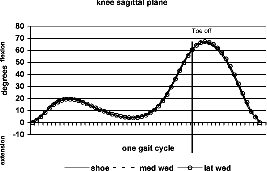
\includegraphics[width=0.8\linewidth]{knee_kinematic.pdf}
    \caption{Actual human knee flexion kinematic during the walking gait~\cite{Nester2003}. We can identify two main phases corresponding to the preparation of the stance phase and the swing phase. The main difference is the amplitude of the motion i.e $<20$\textsuperscript{o}  for the stance phase and $>20$\textsuperscript{o} for the swing phase.}
    \label{fig:human_knee_kinematic}
\end{figure}

We performed a parametric optimization both on the position of the spring ties ($M_T$ and $M_L$) and on its characteristic ($K$, $L_0$, $D_i$, $F_{max}$, $L_{max}$) (see Fig.~\ref{fig:knee_conception}) to try to match the above mentioned criteria. These criteria are modeled as condition on the resultant torque:

\begin{itemize}
    \item $C(\theta=0) < -0.4$: Locking of the knee, where $0.4 N.m$ is the necessary torque to keep the leg straight.
    \item $C(\theta=25 \textsuperscript{o} ) = 0$: Transition between the two behaviors
    \item $C > 0$ if $\theta > 25 deg$: Helps the motor to lift the leg.
    % \item $ max(\abs{C(\theta)}) < \frac{C_{MX-28}}{2}$: The actuator $MX-28$ should always be powerful enough to control the joint motion.
\end{itemize}

\begin{figure}[thpb]
    \centering
    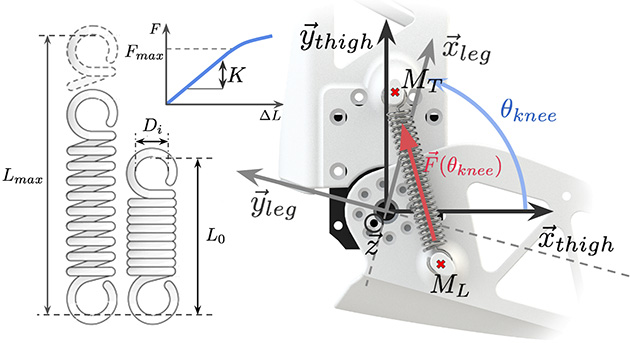
\includegraphics[width=0.95\linewidth]{knee_spring.jpg}
    \caption{Spring parameters to optimized}
    \label{fig:knee_conception}
\end{figure}


The resultant torque $C$ generated by springs in function of the knee flexion $\theta$  ($n_{spring} = 2$) is computed as follow:

\begin{equation}
    C(\theta) = n_{spring} \cdot \overrightarrow{OM_L}{\rvert}_{R_{thigh}} \wedge \overrightarrow{F}(\theta) \cdot \overrightarrow{z}
\end{equation}

with:

\begin{equation}
    \norm{ F(\theta)} = K \cdot \left ( L(\theta) - L_0\right )
\end{equation}

\begin{equation}
    L(\theta) = \quad \norm{ \overrightarrow{M_T M_L}{\rvert}_{R_{thigh}}}\qquad
\end{equation}

\begin{equation}
    \overrightarrow{OM_L}{\rvert}_{R_{thigh}}  = \overrightarrow{OM_L}{\rvert}_{R_{leg}}  \cdot
    \begin{bmatrix}
        cos(\theta) & -sin(\theta) & 0 \\
        sin(\theta) & cos(\theta) & 0 \\
        0 & 0 & 1\\
    \end{bmatrix}
\end{equation}



We use an iterative selection on these criteria to determine the appropriate characteristics for the spring.

\paragraph{Minimizing stresses on the structure} % (fold)
\label{par:minimize_stresses_on_the_structure}

The length of the lever arm is constrained by the dimensions of the legs, resulting in an increase of the force generated by the spring to produce the desired torque on the knee.

By maximizing the following criterion with the constraint $C(\theta=25 \textsuperscript{o} ) = 0$:
\begin{equation}
     c_1 = \frac{C_{max}}{F_{max}^2}
\end{equation}

We were able to determine the ties specific location ($M_T$ and $M_L$), for both minimizing mechanical stress and changing the torque direction for $\theta = 25\textsuperscript{o}$,

{\centering
    $M_T={\left \{2,39,0 \right \}_R}_{thigh}$~$ M_L = {\left \{-12,23,0 \right \}_R}_{leg}$

}
and constraints concerning the springs characteristics:

{\centering
    $L_{min} < 42.6 mm$ ~$L_{max} > 65.12 mm$

}
% paragraph minimize_stresses_on_the_structure (end)

\paragraph{Ties strength} % (fold)
\label{par:ties_strength}

We calculated the minimum diameter of the ties so that it can withstand the constraints imposed by the spring with a beam theory model:
\begin{equation}
    D_{min}= \sqrt[3]{ \frac{32 \times  C_s \times F_{max} \times l_{tie}}{2 \pi \times \sigma_{MaxPolyamide}} }
\end{equation}
By considering Poppy's parameters and a coefficient of safety $C_s = 5$, we
found that the spring must respect the criterion $D_{min} > 6.5 mm$.

% paragraph ties_strength (end)

Considering the desired spring behavior and geometrical conditions, an automatic selection over 720 different springs\footnote{pre-selection of springs in the vanel.com catalogue} was performed. Only 5 springs satisfied all criteria. For the Poppy platform we chose a spring with the following characteristics: $\{ D_i=9.6mm$, $L_0=42mm$, $K=1620N.m^{-1}$, $F_{max}=81.7 N$, $L_{max}=72.8 mm \}$ inducing a resultant behavior shown in Fig.~\ref{fig:knee_feature}. As we can see, even if the torque applied by the spring is quite low ($C_{max} = 0.74 N.m$), the force subjected to spring ties is up to $40N$. The shape of this ties has been optimized using FEA in order to handle the stress.

An illustration of the real behavior is shown in the attached videos\footnote{\url{flowers.inria.fr/IROS2013/poppy_knee.m4v}}.

\begin{figure}[thpb]
    \centering
    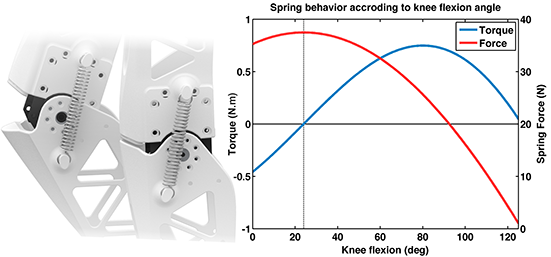
\includegraphics[width=0.95\linewidth]{torque_knee.png}
    \caption{Actual spring behavior for the semi-passive knee. The blue line corresponds to the torque applied by the spring on the leg according to the flexion angle of the knee. The red line corresponds to the force that the spring applied on ties.}
    \label{fig:knee_feature}
\end{figure}


\begin{figure}[!h]
\centering
    \subfloat[][without springs]{\label{fig:knee_wout_spring}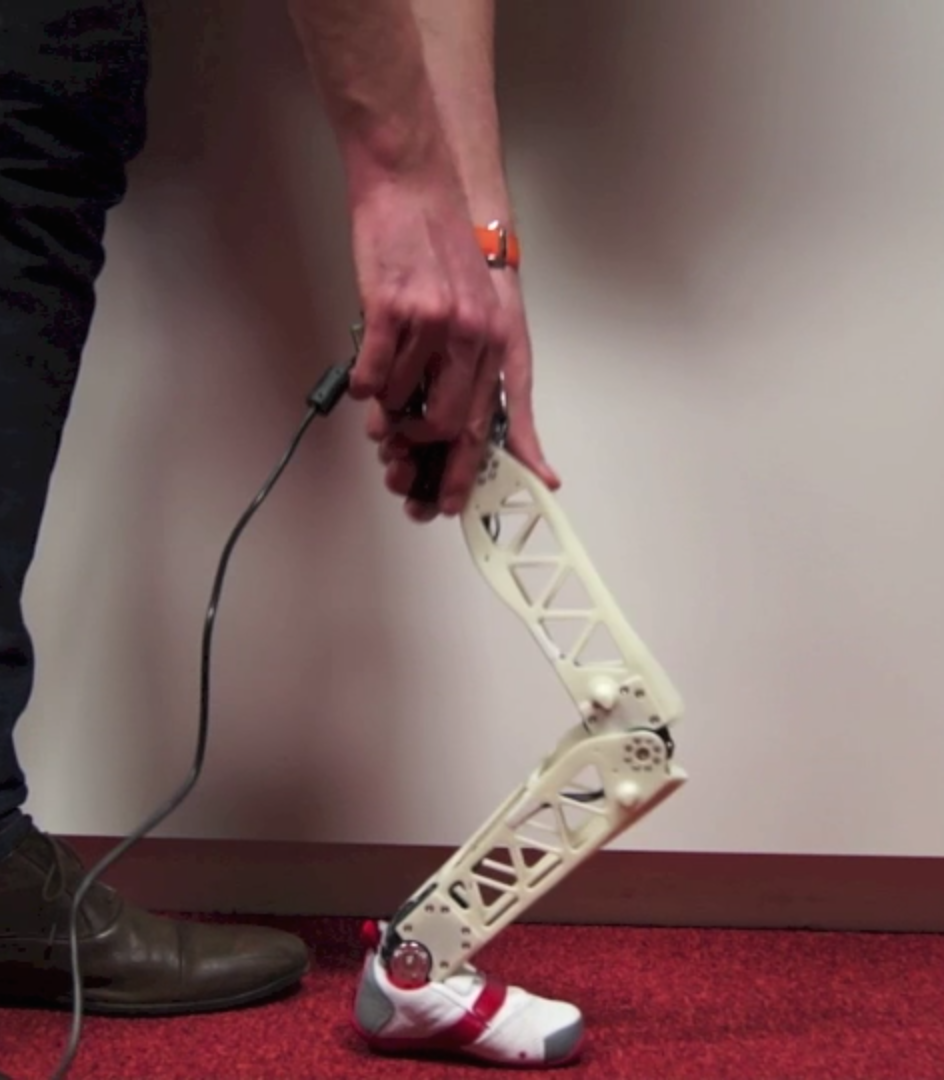
\includegraphics[height=5cm]{knee_wout_spring.png}}
    \hfil
    \subfloat[][with traction spring]{\label{fig:knee_w_spring}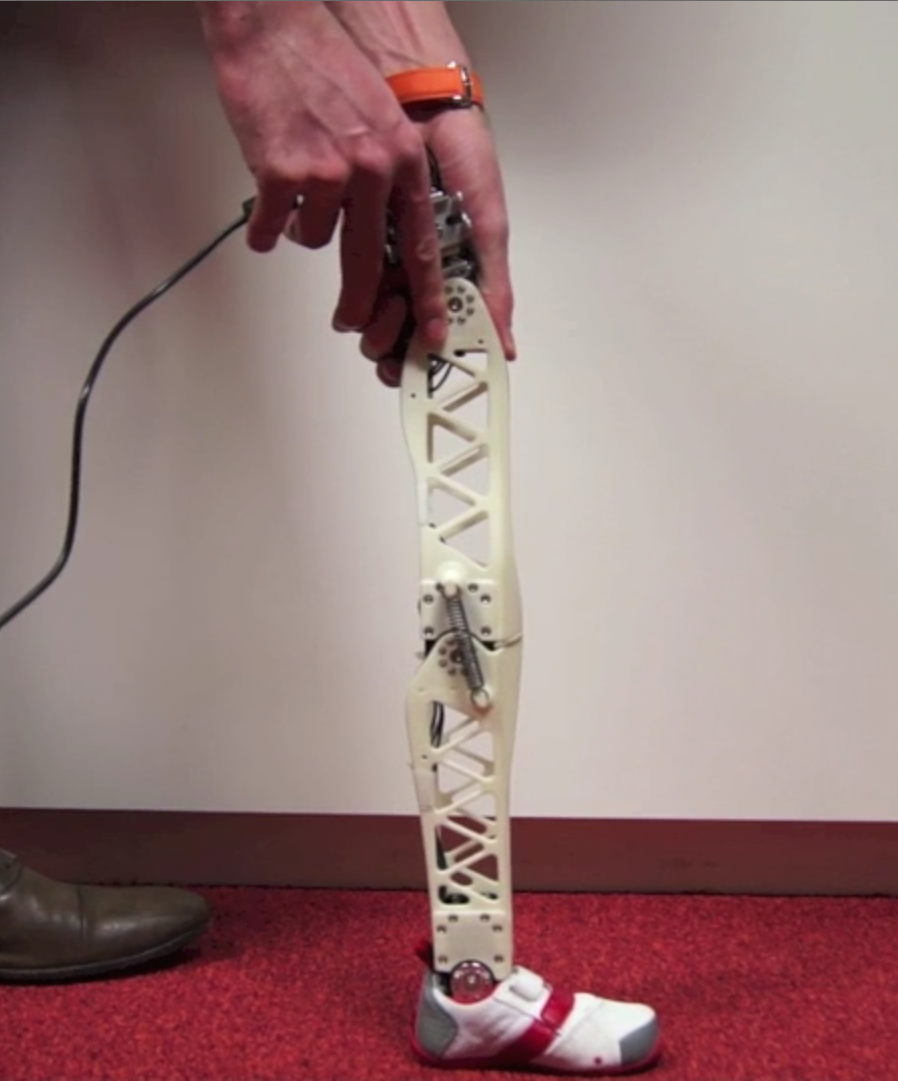
\includegraphics[height=5cm]{knee_w_spring}}
    \caption{Motors fully compliant \url{https://vimeo.com/63839782}}
    \label{fig:}
\end{figure}



\subsection{A multi-articulated trunk} % (fold)

\begin{figure}[!t]
\centering
    \subfloat[][]{\label{fig:frontal_trunk}\includegraphics[width=0.49\linewidth]{trunk_face.png}}
    \hfil
    \subfloat[][]{\label{fig:sagittal_trunk}\includegraphics[width=0.49\linewidth]{trunk_sagittal.png}}
    \caption{These figures illustrate some morphological features of the Poppy humanoid Robot:\newline a) The Poppy's limbs follow the human being proportion as described in~\cite{dufour2005biomecanique}.\newline b) and c) Poppy has an articulated trunk of 5 DoFs which allows more natural and fluid motions while improving the user experience during physical interaction and actively participating to the balance of the robot.}
    \label{fig:poppy_features}
\end{figure}

Poppy uses the bio-inspired trunk system introduced by Acroban. Using five servo-motors, it allows the reproduction of the main DOFs of the human spine. This feature permits the integration of more natural and fluid motion while improving the user experience during physical interaction. In addition, the spine plays a fundamental role in bipedal walking and postural balance by actively participating in the balancing of the robot.

Contrary to the design of the hips, it was not possible here to fit the 5 motors in the frontal plane due to the limited space in the trunk. So to reduce the shifting of the center of gravity to the back of the robot we gradually shifted the upper body to the front. By doing so, we keep the CoG in the support polygon.



\section{Physical and Social interaction} % (fold)



\subsection{The head} % (fold)

\subsection{Underpowered and compliant for safety} % (fold)



\section{Electronic architecture} % (fold)




\section{The control architecture} % (fold)


Right from the beginning of the poppy platform development with started the development of a new python library to control the robot.
Following the hardware guidelines, the pypot library was developed to be robust, versatile and easy to use.

Also, multi-platform, easy-to-use and lightweight are not often associated with ROS.


\subsection{Pypot: a versatile control library} % (fold)

\begin{figure}[tb]
    \begin{center}
        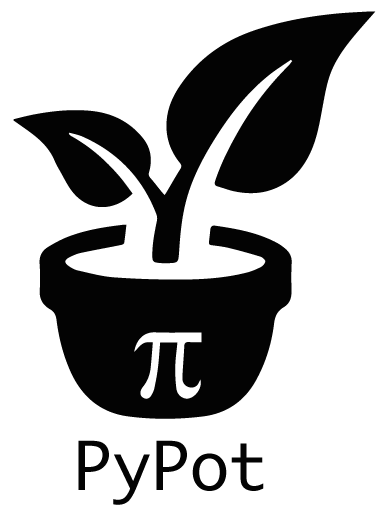
\includegraphics[height=5cm]{PyPot_logo_black_transparentbg.png}
    \end{center}
    \caption{The pypot library logo}
    \label{fig:pypot_logo}
\end{figure}



PyPot is a library developed in the Poppy-project to make it easy and fast to control custom robots based on dynamixel motors. PyPot has been entirely written in Python to allow for fast development, easy deployment and quick scripting by non-necessary expert developers. The serial communication is handled through the standard library and thus allows for rather high performance (10ms sensorimotor loop). It is crossed-platform and has been tested on Linux, Windows and Mac OS. This framework provides different level of abstraction corresponding to different types of use from synchronous low-level motor control to high-level primitives such as walking gait.

directly control robotis motors through a USB2serial device,
define the structure of your particular robot and control it through high-level commands.

\begin{itemize}
    \item Fast sensori-motor loop: it is possible at 100Hz up to 10 motors on the same bus and even more if USB2AX dongle is used.
    \item
\end{itemize}

EASE OF USE!
Synchronizes at 100Hz up to 10 motors on the same bus.
Much more if you use the USB2AX controller.
Handles as many buses as you need and automatically combines them into a single transparent unified interface.
DIFFERENT ACCESS LEVELS
Synchronous/asynchronous low-level motor commands.
Hierarchical high-level primitives.
Remote access (socket or HTTP requests).
PRIMITIVES
Split behaviors into separate primitives.
Creates complex hierarchical primitives from simpler ones.
Automatically combines them at runtime.
PYTHON POWERED
Multi-platform support and easy installation.
Code simple and easy to maintain.
Benefits from numpy/scipy and machine learning libraries.
VARIETY OF SUPPORTED SENSORS
Arduino boards interface.
Kinect connection.
NaturalPoint OptiTrack bridge.
EASY TO EXTEND
REST API to be remotely connected to other softwares.
Software architecture designed to be extended (e.g. new motors, new sensors, new primitives).
FULLY DOCUMENTED!
Tutorial and samples.

\subsection{Why not using ROS ?} % (fold)
One of our main preoccupation is to develop an easy to use research tools.
In this context, we designed pypot to be multi OS compatible.
ROS is a great software but until now, it is really difficult to set up and need a specific Ubuntu version.
Also this software is very greedy which would make its integration difficult in a small robot.

We prefer an interface with ROS.

\subsection{The primitive architecture: The Good, the Bad and the Ugly} % (fold)
The high level design allows the use of primitives.
Primitives are ...

This features is really powerful has it allows to create complex behavior as a sum of simple behavior.


However the interaction between them is tricky and can lead to undesired behavior.



\section{Conclusions} % (fold)

Thanks to the methodology presented in the previous chapter, we were able to develop a first functional version of Poppy in only 4 months.

\section{Limitations} % (fold)



